%%%%%%%%%%%%%%%%%%%%%%%%%%%%%%%%%%%%%%%%%%%%%%%%%%%%%%%%%%%%%%%%%%%%%%%%%%%%%%%%
% AMS Beamer series / Bologna FC / Template
% Andrea Omicini
% Alma Mater Studiorum - Università di Bologna
% mailto:andrea.omicini@unibo.it
%%%%%%%%%%%%%%%%%%%%%%%%%%%%%%%%%%%%%%%%%%%%%%%%%%%%%%%%%%%%%%%%%%%%%%%%%%%%%%%%
%\documentclass[handout]{beamer}\mode<handout>{\usetheme{default}}
%
\documentclass[presentation, 9pt]{beamer}\mode<presentation>{\usetheme{AMSBolognaFC}}
%\documentclass[handout]{beamer}\mode<handout>{\usetheme{AMSBolognaFC}}
%%%%%%%%%%%%%%%%%%%%%%%%%%%%%%%%%%%%%%%%%%%%%%%%%%%%%%%%%%%%%%%%%%%%%%%%%%%%%%%%
\usepackage[T1]{fontenc}
\usepackage{wasysym}
\usepackage{amsmath,blkarray}
\usepackage[minted,most]{tcolorbox}
\usepackage{centernot}
\usepackage{fontawesome}
\usepackage{fancyvrb}
\usepackage{minted}
\usepackage{multicol}
\setminted[scala]{fontsize=\scriptsize,baselinestretch=1,obeytabs=true, tabsize=2}
\usepackage[ddmmyyyy]{datetime}
\setminted{fontsize=\footnotesize}
\renewcommand{\dateseparator}{}
%\renewcommand{\thefootnote}{\fnsymbol{footnote}}
\newcommand{\version}{1}
\usepackage[
	backend=biber,
	citestyle=authoryear-icomp,
	maxcitenames=1,
	bibstyle=numeric]{biblatex}

	\makeatletter

\addbibresource{biblio.bib}
%%%%%%%%%%%%%%%%%%%%%%%%%%%%%%%%%%%%%%%%%%%%%%%%%%%%%%%%%%%%%%%%%%%%%%%%%%%%%%%%
\title[Deep Reinforcement Learning: Intro]
{Deep Reinforcement Learning}
%
\subtitle[Introduction and Hands-on in Simple Environments]
{Introduction and Hands-on in Simple Environments}
%
\author[\sspeaker{Aguzzi}]
{\speaker{Gianluca Aguzzi} \href{mailto:gianluca.aguzzi@unibo.it}{gianluca.aguzzi@unibo.it}}
%
\institute[DISI, Univ.\ Bologna]
{Dipartimento di Informatica -- Scienza e Ingegneria (DISI)\\
\textsc{Alma Mater Studiorum} -- Universit{\`a} di Bologna \\[0.5cm]
\textbf{Talk @} \bold{Fondamenti di Intellingenza Artificiale}}
%
\renewcommand{\dateseparator}{/}
\date[\today]{\today}
%
\AtBeginSection[]
{
  \begin{frame}
  \frametitle{Contents}
  \tableofcontents[currentsubsection, 
	sectionstyle=show/shaded, 
	subsectionstyle=show/shaded]
  \end{frame}
}
\AtBeginSubsection[]
{
  \begin{frame}
  \frametitle{Contents}
  \tableofcontents[currentsubsection, 
	sectionstyle=show/shaded, 
	subsectionstyle=show/shaded]
  \end{frame}
}
%%%%%%%%%%%%%%%%%%%%%%%%%%%%%%%%%%%%%%%%%%%%%%%%%%%%%%%%%%%%%%%%%%%%%%%%%%%%%%%%
\begin{document}
%%%%%%%%%%%%%%%%%%%%%%%%%%%%%%%%%%%%%%%%%%%%%%%%%%%%%%%%%%%%%%%%%%%%%%%%%%%%%%%%

%/////////
\frame{\titlepage}
%/////////
\begin{frame}{Me}
	\begin{columns}
		\begin{column}{0.5\textwidth}
		\centering
		\fbox{
\includegraphics[width=0.5\linewidth]{img/me.jpeg}}
		\\
		\vspace{0.2cm}
		\href{https://github.com/cric96}{\faGithub} \,
		\href{https://stackoverflow.com/users/10295847/gianluca-aguzzi}{\faStackOverflow} \,
		\href{https://www.linkedin.com/in/gianluca-aguzzi-265998170/}{\faLinkedin} \,
		\href{https://www.unibo.it/sitoweb/gianluca.aguzzi}{\faGlobe} \,
		\end{column}
		\begin{column}{0.5\textwidth}
			\begin{itemize}
				\item PhD student in Computer Science and Engineering
				\item Research interests:
				\begin{itemize}
					\item Multi-agent systems
					\item Distributed Collective Intellingence
					\item Deep Learning Learning
					\item Multi-agent Reinforcement Learning
					\item Macro-programming
				\end{itemize}
				\item Lead developer of \href{https://scafi.github.io/}{ScaFi}
				\item Scala Lover \& Functional Programming enthusiast
			\end{itemize}
		\end{column}
	\end{columns}
\end{frame}
%===============================================================================
\section{Introduction}
%===============================================================================
\begin{frame}{Road to \bold{Deep} Reinforcement Learning}
	\begin{block}{Overview}
		\begin{itemize}
		\item \textbf{Reinforcement Learning (RL)} \faArrowRight \, learning how to act in order to maximize a numerical reward signal
		\item Key features:
		\begin{itemize}
			\item \textbf{trial-and-error search} (no supervisor)
			\item \textbf{delayed reward} (no immediate feedback)
		\end{itemize}
	\end{itemize}
	\end{block}
	\begin{block}{Application}
		\begin{multicols}{2}
		\begin{itemize}
			\item Robotics
			\item Game playing
			\item Resource management
			\item Finance
			\item Chatbots
			\item Intelligent transportation systems
		\end{itemize}
		\end{multicols}
	\end{block}

	\begin{alertblock}{Question}
		\centering
		\textbf{Can standard RL (e.q., Q-Learning) solve these complex problems?}		
	\end{alertblock}
\end{frame}
%\subsection{Reinforcement Learning Pitfalls}
\begin{frame}{Reinforcement Learning Pitfalls: Large state space}
\begin{block}{Problem}
	\begin{itemize}
		\item \textbf{State space} \faArrowRight \, set of all possible states
		\item \textbf{State space explosion} \faArrowRight \, the number of states is too large to be stored in memory
	\end{itemize}
\end{block}
\begin{columns}
	\begin{column}{0.5\textwidth}
		
			\begin{block}{Example (Go) \, \href{}{\faLink}}
				\begin{itemize}
					\item $10^{170}$ possible states \bold{(!!!!)}
					\item $10^{80}$ atoms in the universe
					\item $10^{16}$ seconds since the Big Bang
				\end{itemize}
			\end{block}
			\begin{block}{Example (Chess) \, \href{}{\faLink}}
				\begin{itemize}
					\item $10^{46}$ possible states
					\item total space required $\sim$ $10^{35}$ terabytes
				\end{itemize}
			\end{block}
	\end{column}
	\begin{column}{0.5\textwidth}
	\centering
	\fbox{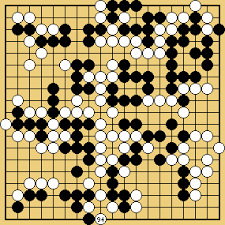
\includegraphics[width=0.67\linewidth]{img/go.png}}
	\end{column}
\end{columns}

\begin{alertblock}{Question}
	\centering
	\textbf{How to deal with large state space?}
\end{alertblock}
\end{frame}

\begin{frame}{Reinforcement Learning Pitfalls: Continous Action Space}
	\begin{block}{Problem}
		\begin{itemize}
			\item \textbf{Action space} \faArrowRight \, set of all possible actions
			\item \textbf{Continous action space} \faArrowRight \, the actions are real numbers (e.g. $[0,1]$) \faArrowRight infinite number of actions
		\end{itemize}
	\end{block}
	\begin{columns}
		\begin{column}{0.5\textwidth}
			\begin{block}{Example (Robotics) \, \href{}{\faLink}}
				\begin{itemize}
					\item \textbf{Action space} \faArrowRight \, the set of all possible joint angles
					\item \textbf{Continous action space} \faArrowRight \, the set of all possible real joint angles
				\end{itemize}
			\end{block}
		\end{column}
		\begin{column}{0.5\textwidth}
			\centering
			\fbox{
\includegraphics[width=0.4\linewidth]{img/robotics}}
		\end{column}
	\end{columns}
	
	\begin{alertblock}{Question}
		\centering
		\textbf{How to deal with continous action space?}
	\end{alertblock}
\end{frame}
\begin{frame}{Reinforcement Learning Pitfalls: Generalization}
\begin{block}{Problem}
	\begin{itemize}
		\item \textbf{Generalization} \faArrowRight \, the ability to perform well on previously unseen environments
		\item Can be also seen as \textbf{transfer learning} \faArrowRight \, the ability to transfer knowledge from one environment to another
		\item \textbf{Generalization gap} \faArrowRight \, the difference between the performance on the training environments and the performance on the test environments
	\end{itemize}
\end{block}
\begin{block}{Example (Go) \, \href{}{\faLink}}
	\begin{itemize}
		\item \textbf{Generalization} \faArrowRight \, the ability to play well with different opponents
		\item \textbf{Generalization gap} \faArrowRight \, the difference between the performance on the training set and the performance on the test set
	\end{itemize}
\end{block}
\begin{alertblock}{Question}
	\centering
	\textbf{How to deal with generalization?}
\end{alertblock}
\end{frame}
%\subsection{Deep Reinforcement Learning Overview}
\begin{frame}{Deep Reinforcement Learning}
	\centering
	\fbox{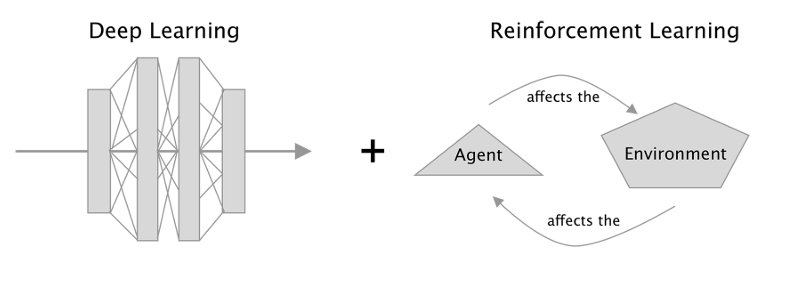
\includegraphics[width=0.7\textwidth]{img/deep-rl.png}}
	\begin{block}{Overview}
		\begin{itemize}
			\item \textbf{Deep Reinforcement Learning (DRL)} \faArrowRight \, the use of deep neural networks to approximate the value function / policy
			%\item Stochastic gradient descent \faArrowRight \, the use of gradient descent to train the neural networks
		\end{itemize}
	\end{block}
	
	\begin{alertblock}{Key features}
		\begin{itemize}
			\item \textbf{value function approximation} (instead of table) \faArrowRight \, \textbf{handle large state space}
			\item \textbf{policy gradient} (instead of Q-Learning) \faArrowRight \, \textbf{handle continous action space}
			\item \textbf{deep neural networks} \faArrowRight \, \textbf{handle generalization} (Representation learning)
		\end{itemize}
	\end{alertblock}
\end{frame}
\begin{frame}{Algorithms types}	
\begin{columns}
	\begin{column}{0.45\textwidth}
		\begin{block}{Value-based}
			\begin{itemize}
				\item the agent learns the value function
				\item \textbf{Example} \faArrowRight \, \emph{Deep Q-Learning}
			\end{itemize}
		\end{block}

		\href{https://www.youtube.com/watch?v=V1eYniJ0Rnk}{\fbox{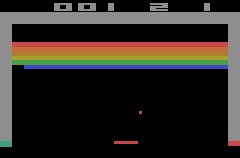
\includegraphics[height=3.5cm]{img/atari}}}
	\end{column}

	\begin{column}{0.45\textwidth}
		\begin{block}{Policy-based}
			\begin{itemize}
				\item the agent learns the policy 
				\item \textbf{Example} \faArrowRight \, REINFORCE, PPO
			\end{itemize}
		\end{block}
		\centering
		\href{https://openai.com/research/openai-baselines-ppo}{\fbox{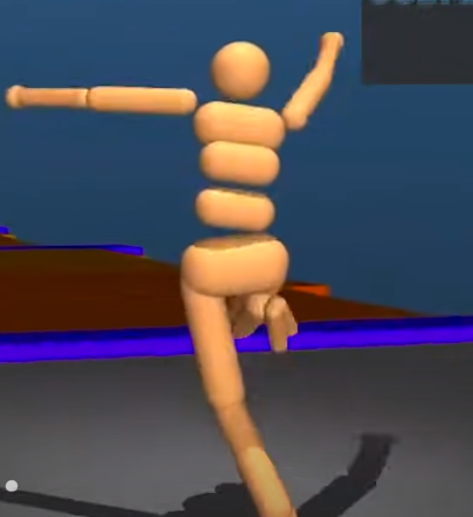
\includegraphics[height=3.5cm]{img/ppo.png}}}
	\end{column}
\end{columns}

\end{frame}
\section{Deep Q-Learning}
\begin{frame}{Deep Q-Learning}
	\centering
	\textbf{Q-Learning but q-function is approximated by a neural network}
	$$ Q(s, a, \theta) \sim Q(s, a) $$
	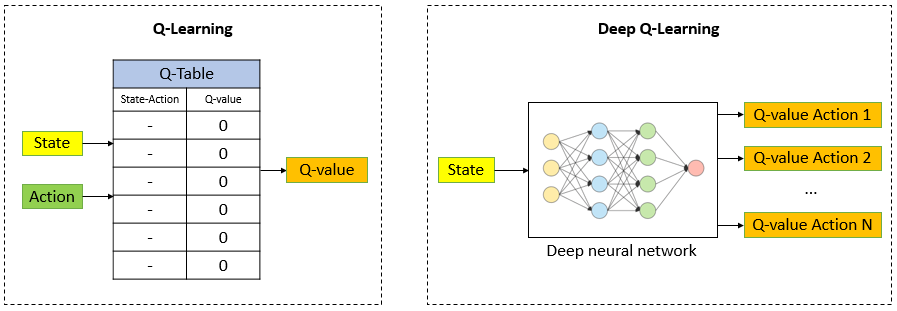
\includegraphics[width=\textwidth]{img/dql-vs-ql-1.png}
\end{frame}

\begin{frame}{Deep Q-Learning}
	\begin{alertblock}{Loss function}
		\begin{itemize}
			\item Bellman equation: $Q(s, a) = (r + \gamma \max_{a'} Q(s', a'))$
			\item Treating $r + \gamma \max_{a'} Q(s', a')$ as a target value
			\item Regression problem: $L(\theta) = (r + \gamma \max_{a'} Q(s', a', \theta) - Q(s, a, \theta))^2$
		\end{itemize}
	\end{alertblock}
	\begin{block}{Issues}
		\begin{itemize}
			\item \textbf{Correlation} \faArrowRight \, the samples are not independent
			\item \textbf{Non-stationary} \faArrowRight \, the target value changes over time
		\end{itemize}
	\end{block}
	\begin{alertblock}{Solutions}
		\begin{itemize}
			\item \textbf{Replay Buffer} \faArrowRight \, store the transitions $(s, a, r, s')$ and sample them randomly
			\item \textbf{Target Network} \faArrowRight \, used to compute the target value
		\end{itemize}
	\end{alertblock}
\end{frame}
\begin{frame}{Deep Q Learning: Replay Buffer}
	\centering
	\fbox{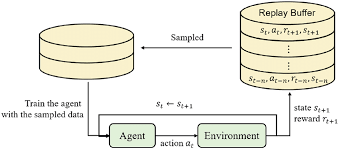
\includegraphics[width=0.5\textwidth]{img/replay-buffer.png}}
	\begin{block}{How}
		\begin{itemize}
			\item Store the transitions $(s, a, r, s')$ in $\mathcal{D}$ of prior experience
			\item During Backpropagation, sample a batch of transitions $(s, a, r, s')$ 
		\end{itemize}
	\end{block}
	\begin{block}{Loss computation}
		\begin{itemize}
			\item Sample a random batch of transitions $(s, a, r, s')$ from $\mathcal{D}$
			\item Compute the target value $y = r + \gamma \max_{a'} Q(s', a', \theta)$
			\item Use the target value to compute the loss $L(\theta) = \mathbb{E}[(y - Q(s, a, \theta))^2]$
		\end{itemize}
	\end{block}
\end{frame}
\begin{frame}{Deep Q Learning: Fixed Target Network}
	\centering
	%\fbox{\includegraphics[width=0.5\textwidth]{img/target-network.png}}
	\begin{block}{How}
		\begin{itemize}
			\item Use a separate network to compute the target value
			\item The target network is updated every $C$ steps
		\end{itemize}
	\end{block}
	\begin{block}{Loss computation}
		\begin{itemize}
			\item Let $\theta^-$ be the parameters of the target network
			\item Sample a random batch of transitions $(s, a, r, s')$ from $\mathcal{D}$
			\item Compute the target value $y = r + \gamma \max_{a'} Q(s', a', \theta^-)$
			\item Use the target value to compute the loss $L(\theta) = \mathbb{E}[(y - Q(s, a, \theta))^2]$
			\item After $C$ steps, update the target network parameters $\theta^- \leftarrow \theta$
		\end{itemize}
	\end{block}
	\begin{alertblock}{Benefits}
		\begin{itemize}
			\item \textbf{Stable} \faArrowRight \, the target value is fixed for $C$ steps, avoiding the non-stationary issue (dipendece on target and prediction cause)
		\end{itemize}
	\end{alertblock}
\end{frame}
\begin{frame}{Deep Q Learning: Epsilon decay}
	\begin{block}{How}
		\begin{itemize}
			\item $\epsilon$ is the probability of selecting a random action
			\item $\epsilon$ is decayed over time (or steps or episodes)
			\item \textbf{(!!!)} Off-policy nature of DQL \faArrowRight \, the agent can learn from random actions
		\end{itemize}
	\end{block}
	\begin{block}{Why}
		\begin{itemize}
			\item \textbf{Exploration vs Exploitation} \faArrowRight \, the agent needs to explore the environment to learn the optimal policy
			\item \textbf{Exploitation} \faArrowRight \, the agent needs to exploit the learned policy to maximize the reward
		\end{itemize}
	\end{block}
	
\end{frame}
\begin{frame}{Deep Q Learning: Algorithm}
	\begin{block}{Algorithm}
		\begin{itemize}
			\item Initialize the replay buffer $\mathcal{D}$
			\item Initialize the target network parameters $\theta^-$
			\item Initialize the Q-network parameters $\theta$
			\item \textbf{for} episode = 1, M \textbf{do}
			\begin{itemize}
				\item Initialize the initial state $s_1$
				\item \textbf{for} t = 1, T \textbf{do}
				\begin{itemize}
					\item With probability $\epsilon$ select a random action $a_t$
					\item otherwise select $a_t = argmax_a Q(s_t, a, \theta)$
					\item Execute action $a_t$ in the environment and observe reward $r_t$ and next state $s_{t+1}$
					\item Store transition $(s_t, a_t, r_t, s_{t+1})$ in $\mathcal{D}$
					\item Sample a random minibatch of transitions $(s, a, r, s')$ from $\mathcal{D}$
					\item Set $y_i = r + \gamma \max_{a'} Q(s', a', \theta^-)$
					\item Perform a gradient descent step on $(y_i - Q(s, a, \theta))^2$ with respect to the network parameters $\theta$
					\item Every $C$ steps reset $\theta^- \leftarrow \theta$
				\end{itemize}
			\end{itemize}
		\end{itemize}
	\end{block}
\end{frame}
\begin{frame}{Deep Q Learning: Extensions and Limits}
	\begin{block}{Limits}
		\begin{itemize}
			\item Works only for discrete action spaces
			\item Sample inefficiencient
			\item Overestimation of the action value due to the max operator
		\end{itemize}
	\end{block}
	\begin{block}{Extensions}
		\begin{itemize}
			\item \textbf{Double DQN} \faArrowRight \, use two separate networks to select and evaluate the action
			\begin{itemize}
				\item Pro: avoid overestimation of the action value
			\end{itemize}
			\item \textbf{Dueling DQN} \faArrowRight \, use two separate networks to estimate the state value and the advantage function
			\begin{itemize}
				\item Pro: better estimation of the action value
			\end{itemize}
			\item \textbf{Prioritized Experience Replay} \faArrowRight \, sample the transitions from the replay buffer according to their TD-error
			\begin{itemize}
				\item Pro: better exploration of the state space
			\end{itemize}
			\item \textbf{Raindow DQN} \faArrowRight \, combination of the previous extensions
		\end{itemize}
	\end{block}

\end{frame}
\section{Hands-On in Python}
\begin{frame}{Deep Reinforcement Learning in Python}
\begin{block}{Components Required}
	\begin{itemize}
		\item \textbf{Environment} \faArrowRight \, the environment in which the agent operates (also called \textit{gym})
		\item \textbf{Neural Network} \faArrowRight \, the neural network used to approximate the Q-function
		\item \textbf{Learning Agent} \faArrowRight \, the agent that learns the optimal policy
	\end{itemize}
\end{block}
\begin{block}{Reference Libraries}
	\begin{itemize}
		\item \textbf{OpenAI Gym} \url{https://gymnasium.farama.org/content/basic_usage/} \faArrowRight for the environment definition
		\item \textbf{PyTorch} \url{https://pytorch.org/} \faArrowRight for the neural network definition
		\item \textbf{Stable Baselines}  \url{https://stable-baselines.readthedocs.io/en/master/} \,faArrowRight for the DRL algorithms
	\end{itemize}
\end{block}
\end{frame}
\begin{frame}{OpenAI Gym}
	\centering
	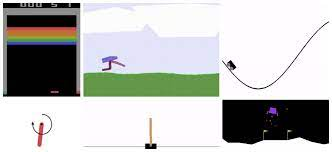
\includegraphics[width=0.4\textwidth]{img/gym}
	\begin{block}{What}
		\begin{itemize}
			\item OpenAI Gym is a toolkit for developing and comparing RL algorithms
			\item It supports teaching agents everything from walking to playing games
			\item It provides a diverse suite of environments that range from easy to difficult and involve many different kinds of data
		\end{itemize}
	\end{block}
	\begin{block}{Why}
		\begin{itemize}
			\item \textbf{Standardized} \faArrowRight \, the environments are standardized \faArrowRight \, algorithms can be compared
			\item \textbf{Easy} \faArrowRight \, the environments are easy to use, so that the focus is on the algorithms
			\item \textbf{Flexible} \faArrowRight \, the environments are flexible, so that new environments can be added
		\end{itemize}
	\end{block}
\end{frame}
\begin{frame}[fragile, allowframebreaks]{OpenAI Gym}
\begin{block}{Main Concepts}
	\begin{itemize}
		\item \texttt{Env} is a Python class with the following methods:
		\begin{itemize}
			\item \texttt{reset()} \faArrowRight \, reset the environment and return the initial state
			\item \texttt{step(action)} \faArrowRight \, execute the \textbf{action} and return the next state, the \textbf{reward} and a boolean flag indicating if the episode is terminated
			\item \texttt{render()} \faArrowRight \, render the environment
			\item \texttt{close()} \faArrowRight \, close the environment
			\item \texttt{action\_space} \faArrowRight \, the action space (i.e. the set of possible actions)
			\item \texttt{observation\_space} \faArrowRight \, the observation space (i.e., the set of possible observations)
		\end{itemize}
		\item \texttt{Env} is a \textbf{black box} \faArrowRight \, the agent can only interact with it through the methods
	
	\end{itemize}
\end{block}
\begin{block}{Typical usage}
\begin{minted}{python}
import gym
env = gym.make('your-env')
env.reset()
for _ in range(episodes):
	env.render()
	env.step(env.action_space.sample())
env.close()
\end{minted}
\end{block}
\begin{block}{Environment Definition}
\begin{minted}{python}

class MyEnv(gym.Env):
	metadata = {'render.modes': ['human']}
	def __init__(self):
		## Init observation, action spaces
	def step(self, action):
		# Execute one time step within the environment, 
		# return observation, reward, done, info
		...
	def reset(self):
		# Reset the state of the environment to an initial state
		...
	def render(self, mode='human', close=False):
		# Render the environment to the screen
		...
	\end{minted}

\end{block}

\end{frame}

\begin{frame}{PyTorch}
	%\centering
	%\includegraphics[width=0.4\textwidth]{img/pytorch}
	\begin{block}{What}
		\begin{itemize}
			\item PyTorch is an open source machine learning framework
			\item It provides a flexible and efficient library for deep learning
			\item It provides a seamless path from research prototyping to production deployment
		\end{itemize}
	\end{block}
	\begin{block}{Why}
		\begin{itemize}
			\item \textbf{Pythonic} \faArrowRight \, the code is Pythonic \faArrowRight \, it is easy to use
			\item \textbf{Dynamic} \faArrowRight \, the code is dynamic \faArrowRight \, it is easy to debug
			\item \textbf{Fast} \faArrowRight \, the code is fast \faArrowRight \, it is easy to scale
		\end{itemize}
	\end{block}
\end{frame}
\begin{frame}{PyTorch -- Super-fast overview}
	\begin{block}{Tensors}
		\begin{itemize}
			\item \texttt{torch.Tensor} is the central class of the package
			\item \texttt{torch.Tensor} is a multi-dimensional matrix containing elements of a single data type
			\item \texttt{torch.Tensor} provides a lot of methods for manipulating the data
		\end{itemize}
	\end{block}
	\begin{block}{Autograd}
		\begin{itemize}
			\item \texttt{torch.autograd} is a package for automatic differentiation
			\item \texttt{torch.autograd} uses a tape-based system for automatic differentiation
		\end{itemize}
	\end{block}
	\begin{block}{Neural Networks}
		\begin{itemize}
			\item \texttt{torch.nn} is a package for building neural networks
			\item \texttt{torch.nn} provides classes and functions implementing neural networks
			\item \texttt{torch.nn} provides a lot of modules for building neural networks
		\end{itemize}
	\end{block}
\end{frame}
\begin{frame}[fragile]{PyTorch -- API Usage}
\begin{multicols}{2}
\begin{minted}{python3}
## Main imports
import torch
import torch.nn as nn
import torch.nn.functional as F
import torch.optim as optim

# Create a tensor
x = torch.tensor(
	[1, 2, 3], 
	dtype=torch.float32
)

# Create a neural network
class Net(nn.Module):
	def __init__(self):
		super(Net, self).__init__()
		self.fc1 = nn.Linear(10, 20)
		self.fc2 = nn.Linear(20, 10)
	def forward(self, x):
		x = F.relu(self.fc1(x))
		x = self.fc2(x)
		return x


## Network initialization
net = Net()

# Create an optimizer
optimizer = optim.SGD(
	net.parameters(), 
	lr=0.01, 
	momentum=0.9
)

# Create a loss function
criterion = nn.MSELoss()
\end{minted}

\begin{minted}{python}
# Perform a forward pass
output = net(x)

# Training loop
for _ in range(epochs):
	# Zero the gradients
	optimizer.zero_grad()
	# Compute the loss
	loss = criterion(output, target)
	# Perform a backward pass
	loss.backward()
	# Update the weights
	optimizer.step()

\end{minted}
\end{multicols}
\end{frame}
\begin{frame}{Stable Baselines 3}
	\begin{block}{What}
		\begin{itemize}
			\item Stable Baselines 3 is a set of reliable implementations of reinforcement learning algorithms
			\item Stable Baselines 3 is a fork of Stable Baselines 2
			\item Stable Baselines 3 is based on PyTorch
		\end{itemize}
	\end{block}
	\begin{block}{Why}
		\begin{itemize}
			\item State-of-the-art implementations of reinforcement learning algorithms
			\item Tested and documented codebase
			\item Easy to use, easy to extend
		\end{itemize}
	\end{block}
	\begin{block}{Main concepts}
		\begin{itemize}
			\item \textbf{Policy} \faArrowRight \, the agent's behavior
			\item \textbf{Environment} \faArrowRight \, the task to be solved
			\item \textbf{Algorithm} \faArrowRight \, the algorithm to train the agent
		\end{itemize}
	\end{block}
\end{frame}
\begin{frame}{Stable Baselines 3 -- Usage Overview}
	\begin{block}{Create an environment}
		\begin{itemize}
			\item \texttt{env = gym.make('CartPole-v1')}
		\end{itemize}
	\end{block}
	\begin{block}{Create a policy}
		\begin{itemize}
			\item \texttt{policy = MlpPolicy(env.observation\_space, env.action\_space)}
			\item \texttt{policy = CnnPolicy(env.observation\_space, env.action\_space)}
		\end{itemize}
	\end{block}
	\begin{block}{Create an algorithm}
		\begin{itemize}
			\item \texttt{model = PPO(policy, env, verbose=1)}
			\item \texttt{model = A2C("MlpPolicy", env, verbose=1)}
			\item \texttt{model = DQN(policy, env, verbose=1)}
		\end{itemize}
	\end{block}
	\begin{block}{Train the agent}
		\begin{itemize}
			\item \texttt{model.learn(total\_timesteps=10000)}
		\end{itemize}
	\end{block}
\end{frame}
\section{Conclusion}
\begin{frame}{Conclusion}
	\begin{block}{What we have learned}
		\begin{itemize}
			\item Deep Reinforcement Learning is a powerful tool for solving complex tasks
			\item Deep Q Learning is a simple yet effective algorithm for solving reinforcement learning tasks
		\end{itemize}
	\end{block}
	\begin{exampleblock}{Just a scratch on the surface}
		\begin{itemize}
			\item Deep Reinforcement Learning is a very active research field
			\item There are a lot of algorithms and techniques to learn
			\item There are a lot of interesting applications to explore
		\end{itemize}
	\end{exampleblock}
	\begin{block}{Resources}
		\begin{itemize}
			\item \citetitle*{10.5555/3312046}: intro to Reinforcement Learning (reference book)
			\item \citetitle*{zai2020deep}: pratice-oriented book on Deep Reinforcement Learning
			\item \citetitle*{graesser2019foundations}: intro to Deep Reinforcement Learning
		\end{itemize}
	\end{block}
\end{frame}
%===============================================================================
\section*{}
%===============================================================================

%/////////
\frame{\titlepage}
%/////////

%===============================================================================
\section*{\refname}
%===============================================================================

%%%%
\setbeamertemplate{page number in head/foot}{}
%/////////
\begin{frame}[c,noframenumbering, allowframebreaks]{\refname}
%\begin{frame}[t,allowframebreaks,noframenumbering]{\refname}
	\tiny
	\nocite{*}
	\printbibliography
\end{frame}
%/////////

%%%%%%%%%%%%%%%%%%%%%%%%%%%%%%%%%%%%%%%%%%%%%%%%%%%%%%%%%%%%%%%%%%%%%%%%%%%%%%%%
\end{document}
%%%%%%%%%%%%%%%%%%%%%%%%%%%%%%%%%%%%%%%%%%%%%%%%%%%%%%%%%%%%%%%%%%%%%%%%%%%%%%%%
